\documentclass{article}
\usepackage{parskip}
\usepackage{amsmath}
\usepackage{amsfonts}
\usepackage{bm}
\usepackage{tikz}

\usepackage[sorting=none]{biblatex} % Imports biblatex package
\addbibresource{references.bib} % Import the bibliography file

\title{Expected loss derviation from Osborne 2009 GPGO article}
\author{Mazin Abdelghany, MD, MS}
\date{3 December 2025}

\begin{document}

\maketitle

\section{Problem statement}

In 2009, Osborne el al. introduced a novel Bayesian approach to global optimization using Gaussian processes \cite{osborne2009gaussian}. In Section 3.1, they derive an analytical expression for a new loss function to determine where best to evaluate a function being optimized using Bayesian optimization. They call this new loss the Bayesian expected loss criterion.

The article sets up the problem as such:

Suppose $(\bm{x}_0, \bm{y}_0)$ are the function evaluations gathered thus far and define $\eta := \min\bm{y}_0$. Given this, we can define the loss of evaluating the function one last time at $x$ and its returning $y$
\[
\lambda(y) := \begin{cases}
y; \quad y < \eta \\
n; \quad y \ge \eta
\end{cases}
\]
The loss at the new observed minimum is $\min(y, \eta)$. The analytic form is then dervied
\[ 
\Lambda_1(x\,|\,I_0) := \int \lambda(y)\cdot p(y \, | \, x, I_0) \, dy = \sum_{i\in S} \rho_i V_i(x \, | \, I_0)
\]
$V_i(x \, | \, I_0)$ is then shown to be
\begin{align*}
V_i(x\,|\,I_0) &:= \eta \int_{\eta}^\infty \mathcal{N}(y; m_i, C_i) \, dy + \int_{-\infty}^{\eta} y\,\mathcal{N}(y; m_i, C_i)\,dy\\
&=\eta + (m_i - \eta)\Phi(\eta; m_i, C_i) - C_i\mathcal{N}(\eta; m_i, Ci)
\end{align*}
Where $m_i$ is $m_i(y|I_0)$---the mean function---and $C_i$ is $C_i(y|I_0)$---the covariance function, with notation sometimes seen as $k(y_0,y\,|\,I_0)$.

\section{Derivation}

We focus on this derivation of $V_i(x \, | \, I_0)$. Our integral must be split at the critical value $\eta$. When $y<\eta$, $\lambda(y)=y$ and when $y\ge\eta$, $\lambda(y)=\eta$. Calling $\Lambda_1(x\,|\,I_0) = \mathbb{E}[\lambda(y)]$ and making explicit that we are integrating over $y$,
\[
\mathbb{E}[\lambda(y)] := \int_{y=-\infty}^{y=\eta} y\cdot p(y \,| \,x, I_0) \, dy + \int_{y=\eta}^{y=\infty} \eta\cdot p(y \,| \,x, I_0) \, dy
\]
Note that $p(y \,| \,x, I_0)$ is driven by the Gaussian process!
\[
p(y \,| \,x, I_0) = \mathcal{N}\big(y; m(y\,|\,I_0), C_i(y|I_0)\big)
\]

Plugging this into the integrals, we get 
\begin{multline*}
\mathbb{E}[\lambda(y)] = \int_{-\infty}^{\eta} y\cdot \mathcal{N}\big(y; m(y\,|\,I_0), C_i(y|I_0)\big) \, dy \\ 
+ \int_{\eta}^{\infty} \eta\cdot \mathcal{N}\big(y; m_i(y\,|\,I_0), C_i(y|I_0)\big) \, dy
\end{multline*}

Let us work on each integral at a time. We can call the first integral $A$ and the second integral $B$. 

\subsection{Integral $B$}
Starting with $B$,
\[
B = \int_{\eta}^{\infty} \eta\cdot \mathcal{N}\big(y; m_i(y\,|\,I_0), C_i(y|I_0)\big) \, dy
\]
Pulling out the $\eta$ as the integral is with respect to $y$ and replacing $m_i(y\,|\,I_0)$ and $C_i(y|I_0)$ with $\mu$ and $\sigma^2$, respectively, for notational simplicity.
\[
B = \eta \int_{\eta}^{\infty} \mathcal{N}(y; \mu, \sigma^2) \, dy
\]
Notice here that we are integrating the pdf of the normal distribution, which can be calculated using its cdf, $\Phi(\cdot)$. All that is needed to replace the intergral with $\Phi(\cdot)$ is to notice that the integral from a value $x$ to infinity is equal to the integral of 1 minus the integral of negative infinity to that value.
\newline
\newline
\newline
\begin{minipage}{0.5\textwidth}
\centering
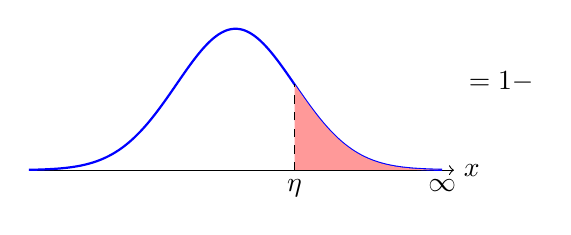
\begin{tikzpicture}[scale=0.75]
    % Define the standard normal density
    \def\phi(#1){6 * 1/sqrt(2*pi) * exp(-(#1)^2 / 2)}

    % Axis
    \draw[->] (-3.5,0) -- (3.7,0) node[right] {$x$};

    % Draw the standard normal curve
    \draw[thick,blue,domain=-3.5:3.5,samples=200]
        plot (\x, {\phi(\x)});

    % Shade the tail area from eta to infinity
    \begin{scope}
        \clip (1,0) rectangle (3.5,2);
        \fill[red!40,domain=-3.5:3.5,samples=200]
            plot (\x, {\phi(\x)});
    \end{scope}

    % Draw vertical line for eta
    \draw[dashed] (1,0) -- (1,{\phi(1)});

    % Label eta
    \node[below] at (1,0) {$\eta$};

    % Add = 1 minus
    \node at (4.5,1.5) {$=1-$};

    % Label infinity
    \node[below] at (3.5,0) {$\infty$};
\end{tikzpicture}
\end{minipage}
\begin{minipage}{0.5\textwidth}
\centering
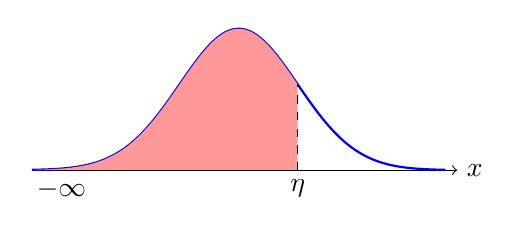
\begin{tikzpicture}[scale=0.75]
    % Define the standard normal density
    \def\phi(#1){6 * 1/sqrt(2*pi) * exp(-(#1)^2 / 2)}

    % Axis
    \draw[->] (-3.5,0) -- (3.7,0) node[right] {$x$};

    % Draw the standard normal curve
    \draw[thick,blue,domain=-3.5:3.5,samples=200]
        plot (\x, {\phi(\x)});

    % Shade the tail area from minus infty to eta
    \begin{scope}
        \clip (-3.5,0) rectangle (1,2.39);
        \fill[red!40,domain=-3.5:3.5,samples=200]
            plot (\x, {\phi(\x)});
    \end{scope}

    % Draw vertical line for eta
    \draw[dashed] (1,0) -- (1,{\phi(1)});

    % Label eta
    \node[below] at (1,0) {$\eta$};

    % Label infinity
    \node[below] at (-3,0) {$-\infty$};
\end{tikzpicture}
\end{minipage}
\newline
\newline
Therefore,
\begin{align*}
B&=\eta \left( 1-\int_{-\infty}^\eta\mathcal{N}(y; \mu, \sigma^2)\,dy \right)\\
&=\eta(1-\Phi(\eta; \mu, \sigma^2))
\end{align*}
\subsection{Integral $A$}
Now, we move to integral $A$:
\[
A=\int_{-\infty}^{\eta} y\cdot \mathcal{N}\big(y; m(y\,|\,I_0), C_i(y|I_0)\big) \, dy
\]
Substituting the pdf of the normal distribution
\[
A=\int_{-\infty}^{\eta} y\cdot \frac{1}{\sqrt{2\pi\sigma^2}} \cdot \exp\left\{ -\frac{1}{2} \left(\frac{y-\mu}{\sigma}\right)^2 \right\}\, dy
\]
Making the substitution $z=\frac{y-\mu}{\sigma}$,
\begin{align*}
dz &= d\left( \frac{y-\mu}{\sigma} \right)\\
&=d\left( \frac{y}{\sigma} -  \frac{\mu}{\sigma}\right)\\
&=\frac{1}{\sigma} dy\\
\sigma \cdot dz &= dy
\end{align*}
We also have to substitute $y$, which is $\sigma z + \mu$ by simple rearrangement.

Plugging in $z$ for $y$,
\[
A=\int_{-\infty}^{\eta} (\sigma z + \mu)\cdot \frac{1}{\sqrt{2\pi\sigma^2}} \cdot \exp\left\{ -\frac{1}{2} z^2 \right\}\, \sigma \cdot dz
\]
The limits of integration also need to be changed. When $y=\infty$,
\begin{align*}
z &= \frac{y-\mu}{\sigma}\\
&= \frac{-\infty-\mu}{\sigma}\\
&=-\infty
\end{align*}
And when $y=\eta$,\
\begin{align*}
z &= \frac{\eta-\mu}{\sigma}
\end{align*}
Thus,
\[
A=\int_{-\infty}^{\frac{\eta-\mu}{\sigma}} (\sigma z + \mu)\cdot \frac{1}{\sqrt{2\pi\sigma^2}} \cdot \exp\left\{ -\frac{1}{2} z^2 \right\}\, \sigma \cdot dz
\]
Pulling out the constant and rearranging the sigma,
\[
A=\frac{1}{\sqrt{2\pi\sigma^2}} \int_{-\infty}^{\frac{\eta-\mu}{\sigma}} \sigma(\sigma z + \mu)\cdot \exp\left\{ -\frac{1}{2} z^2 \right\}\,  dz
\]
Mutliplying out,
\begin{align*}
A&=\frac{1}{\sqrt{2\pi\sigma^2}} \int_{-\infty}^{\frac{\eta-\mu}{\sigma}} \sigma(\sigma z + \mu)\cdot \exp\left\{ -\frac{1}{2} z^2 \right\}\,  dz\\
&=\frac{1}{\sqrt{2\pi\sigma^2}} \int_{-\infty}^{\frac{\eta-\mu}{\sigma}} (\sigma^2 z + \sigma\mu)\cdot \exp\left\{ -\frac{1}{2} z^2 \right\}\,  dz\\
&=\frac{1}{\sqrt{2\pi\sigma^2}} \left[ \int_{-\infty}^{\frac{\eta-\mu}{\sigma}} \sigma^2 z\exp\left\{ -\frac{1}{2} z^2 \right\} + \sigma\mu \exp\left\{ -\frac{1}{2} z^2 \right\}\,  dz \right]
\end{align*}
Distributing the constant $\frac{1}{\sqrt{2\pi\sigma^2}}$ and the integral,
\[
A=\frac{1}{\sqrt{2\pi\sigma^2}} \int_{-\infty}^{\frac{\eta-\mu}{\sigma}} \sigma^2 z\exp\left\{ -\frac{1}{2} z^2 \right\}\,dz + \frac{1}{\sqrt{2\pi\sigma^2}}\int_{-\infty}^{\frac{\eta-\mu}{\sigma}} \sigma\mu \exp\left\{ -\frac{1}{2} z^2 \right\}\,  dz
\]
We can split this integrals again,
\begin{align*}
A_1 = \frac{1}{\sqrt{2\pi\sigma^2}} \int_{-\infty}^{\frac{\eta-\mu}{\sigma}} \sigma^2 z\exp\left\{ -\frac{1}{2} z^2 \right\}\,dz &&
A_2 =\frac{1}{\sqrt{2\pi\sigma^2}}\int_{-\infty}^{\frac{\eta-\mu}{\sigma}} \sigma\mu \exp\left\{ -\frac{1}{2} z^2 \right\}\,  dz
\end{align*}
Taking the first integral $A_1$,
\begin{align*}
A_1 &= \frac{1}{\sqrt{2\pi\sigma^2}} \int_{-\infty}^{\frac{\eta-\mu}{\sigma}} \sigma^2 z\exp\left\{ -\frac{1}{2} z^2 \right\}\,dz\\
&= \frac{\sigma^2}{\sqrt{2\pi\sigma^2}} \int_{-\infty}^{\frac{\eta-\mu}{\sigma}}  z\exp\left\{ -\frac{1}{2} z^2 \right\}\,dz
\end{align*}
This integral can be solved using $u$-substitution with $u = -\frac{1}{2} z^2$.
\[
A_1 = \frac{\sigma^2}{\sqrt{2\pi\sigma^2}}\left[ -\exp \left\{ -\frac{1}{2} z^2 \right\} \Bigg|_{-\infty}^{\frac{\eta-\mu}{\sigma}} \right]
\]
At minus infinity, the above evaluates to 0. Thus, we have
\begin{align*}
A_1 &= \frac{\sigma^2}{\sqrt{2\pi\sigma^2}} -\exp \left\{ -\frac{1}{2} \left(\frac{\eta-\mu}{\sigma}\right)^2 \right\}\\
&=-\sigma^2\underbrace{\frac{1}{\sqrt{2\pi\sigma^2}} \exp \left\{ -\frac{1}{2} \left(\frac{\eta-\mu}{\sigma}\right)^2 \right\}}_{\text{pdf of normal}}\\
&= -\sigma^2\mathcal{N}(\eta; \mu, \sigma^2)
\end{align*}
Now for integral $A_2$,
\begin{align*}
A_2&=\frac{1}{\sqrt{2\pi\sigma^2}}\int_{-\infty}^{\frac{\eta-\mu}{\sigma}} \sigma\mu \exp\left\{ -\frac{1}{2} z^2 \right\}\,  dz\\
&=\sigma\mu\frac{1}{\sqrt{2\pi\sigma^2}}\underbrace{\int_{-\infty}^{\frac{\eta-\mu}{\sigma}}  \exp\left\{ -\frac{1}{2} z^2 \right\}}_{\text{the error function}}\,  dz
\end{align*}
The general form for the integral of the error function is
\[
\int \exp\{-ax^2\}\,dx=\frac{1}{2}\sqrt{\frac{\pi}{a}}\cdot\text{erf}(\sqrt{a}x)
\]
Using this, we complete the above integral as,
\[
A_2=\sigma\mu \frac{1}{\sqrt{2\pi\sigma^2}} \left( \frac{1}{2}\cdot \sqrt{\frac{\pi}{1/2}} \cdot \text{erf} \left(\sqrt{\frac{1}{2}} \cdot z \right) \Bigg|_{-\infty}^{\frac{\eta-\mu}{\sigma}} \right)
\]
The limit as $z\to-\infty$ of the error function is -1. Thus, we have
\begin{align*}
A_2 &=\sigma\mu \frac{1}{\sqrt{2\pi\sigma^2}} \left( \frac{1}{2}\cdot \sqrt{\frac{\pi}{1/2}} \cdot \text{erf} \left(\sqrt{\frac{1}{2}} \cdot \frac{\eta-\mu}{\sigma} \right) -- \frac{1}{2}\cdot \sqrt{\frac{\pi}{1/2}}\right)\\
&=\sigma\mu \frac{1}{\sqrt{2\pi\sigma^2}} \left( \frac{1}{2}\cdot \sqrt{2\pi} \cdot \text{erf} \left(\frac{1}{\sqrt{2}} \cdot \frac{\eta-\mu}{\sigma} \right) +\frac{1}{2}\cdot \sqrt{2\pi}\right)
\end{align*}
Pull the $\sqrt{2\pi}$ all the way out,
\[
A_2 = \sigma\mu \frac{1}{\sqrt{2\pi\sigma^2}}\cdot \sqrt{2\pi} \left( \frac{1}{2}\text{erf} \left(\frac{1}{\sqrt{2}} \cdot \frac{\eta-\mu}{\sigma} \right) +\frac{1}{2}\right)
\]
Pull the $\frac{1}{2}$, but keep it within the paretheses. Also note that $\sqrt{2\pi}$ cancels and $\sigma$ cancels with $1/\sigma^2$ leaving $\mu$ alone out front,
\[
A_2 = \mu \left( \frac{1}{2} \left(1+\text{erf} \left(\frac{1}{\sqrt{2}} \cdot \frac{\eta-\mu}{\sigma} \right) \right)\right)
\]
Finally, we can use the definition of the cdf of the normal distribution,
\[
\Phi\left(x; \mu, \sigma^2\right) = \frac{1}{2} \left(1 + \text{erf}\left(\frac{x-\mu}{\sqrt{2}\sigma}\right)\right)
\]
So,
\[
A_2 = \mu\Phi\left(\eta; \mu, \sigma^2\right)
\]
Combining the two, we get
\[
A =-\sigma^2\mathcal{N}(\eta; \mu, \sigma^2)+ \mu\Phi\left(\eta; \mu, \sigma^2\right)
\]
Adding this to $B$,
\begin{align*}
\mathbb{E}[\lambda(y)] &= \eta(1-\Phi(\eta; \mu, \sigma^2))-\sigma^2\mathcal{N}(\eta; \mu, \sigma^2)+ \mu\Phi\left(\eta; \mu, \sigma^2\right)\\
&=\eta + \mu\Phi\left(\eta; \mu, \sigma^2\right)- \eta\Phi(\eta; \mu, \sigma^2)-\sigma^2\mathcal{N}(\eta; \mu, \sigma^2)\\
&=\eta + (\mu - \eta) \Phi(\eta; \mu, \sigma^2)-\sigma^2\mathcal{N}(\eta; \mu, \sigma^2)
\end{align*}
Substituting back in $m_i$ for $\mu$ and $C_i$ for $\sigma^2$, we can finally right,
\[
\mathbb{E}[\lambda(y)] = \eta + (m_i - \eta) \Phi(\eta; m_i, C_i)-C_i\mathcal{N}(\eta; m_i, C_i).  \quad \square
\]






















\printbibliography

\end{document}